\textbf{4-1} 试求 $1\mathrm{mol}$ 范德瓦耳斯气体由温度 $T_{1}$ ，体积 $V_{1}$ 自由膨胀到体积 $V_{2}$ 时熵的增量，设气体的 $C_V, a, b$ 均为已知的常量。
\vfill

\textbf{4-2} 1 mol氧气在节流过程中体积由高压一边的 $4.0 \times 10^{-3} \, \mathrm{m}^{3}$ 增大到低压一边的 $1.2 \times 10^{-2} \, \mathrm{m}^{3}$ 。已知氧气为范德瓦耳斯气体，范氏常量为 $a = 0.138 \, \mathrm{N \cdot m^{4}/mol^{2}}, b = 3.2 \times 10^{-5} \, \mathrm{m}^{3}/\mathrm{mol}$ ，摩尔定体热容量恒定，为 $C_{V} = 20.8 \, \mathrm{J/(mol \cdot K)}$ 。试计算节流过程前后氧气的温度变化。
\vfill

\newpage
\textbf{4-3} 一定量的乙醚封装在玻璃管内，一部分呈液态，另一部分呈气态，管内无其他杂质。若管内体积恰好为这些乙醚的临界体积，那么在缓慢加热到临界温度时，因气、液两相不再有差别而使液面消失，这就是临界现象的演示实验。假设1mol乙醚的状态方程为 $\left(p+\frac{a}{V^{2}}\right)(V-b)=RT$ ，即为范德瓦耳斯方程，如热图4-3-1所示。

1.已知乙醚的摩尔临界体积为 $V_{K}$ ，在温度为 $T$，压强为饱和蒸汽压时，气相和液相的摩尔体积为 $V_{g}$ 和 $V_{l}$ 。试确定在该温度时玻璃管中气相和液相各占总体积的百分比 $B_{g}$ 和 $B_{l}$ 。

2.在 $V_{g} \gg V_{l}$ 的条件下，试用 $a, b, T$ 来表述 $V_{l}$ 。

3.若在 $20^{\circ}$C 封装乙醚，那么应取 $B_{l}$ 为何值? 已知乙醚临界点的 $T_{K}=466.95\ \mathrm{K}, p_{K}=34.60\ \mathrm{atm}$ 。

\begin{center}
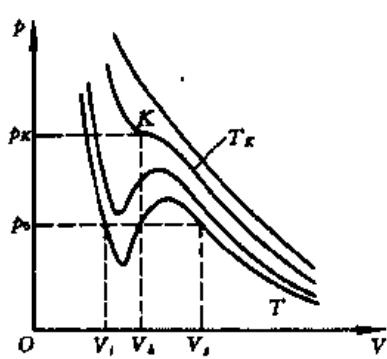
\includegraphics[width=0.2\textwidth]{figures/热图4-3-1.jpg}
\end{center}
\vfill
\newpage

\textbf{4-4} 一种所谓的第二类永动机装置如热图4-4-1所示。图中水平放置的大容器密封但与大气导热，容器左侧A处被围出一个毛细管区域，上方直通容器顶部，右方是实物B，B的外面有相当大的空间 C。图中 D 为一导通管，内有活塞 E 可以无摩擦地左右移动。F 和 G 是两个活门，F 可在一定的压差作用下打开，直到压差几乎为零时才关闭；G 则在一定的压差作用下关闭，直到压差几乎为零时又打开，使 D 与 C 导通。图中水平虚线区域代表某种液体，它与图中所有固体部分均为完全润湿，空白部分只有该液体的饱和蒸汽。

设计者依据：第一，图中用点标出的两处饱和蒸汽压 $p_{1}$ 和 $p_{2}$ 相同。第二，气体内部因高度差引起的附加压强。推证出该装置能往复地从单一热源（大气）吸取热量全部转化为机械功，而不产生其他影响。

1.试完成设计者的推证过程。

2.通过对这个永动机装置的否定，导出 $p_1$ 与 $p_2$ 之间的定量关系，所需参量可自行设取。

\vfill

\newpage
\textbf{4-5} 如热图4-5-1，在一根两端开口、内直径为 $1.0\mathrm{mm}$ 的圆柱形毛细管中，滴入一滴水，然后将它竖直放置。若这滴水在毛细管中分别形成 $1.\, 2.00\mathrm{cm}$，$2.\, 4.00\mathrm{cm}$，$3.\, 2.98\mathrm{cm}$ 的水柱。试问在这三种情况下水柱下端的液面是平面，还是向液体内部凹陷的或向液体外部凸出的曲面？设毛细管能完全润湿水，已知水的表面张力系数 $\alpha = 0.073\mathrm{N / m}$ 。
\begin{center}
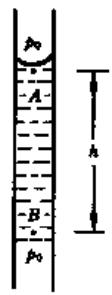
\includegraphics[width=0.08\textwidth]{figures/热图4-5-1.jpg}
\end{center}
\vfill

\textbf{4-6} 如热图4-6-1，有一总长度为 $L$ ，粗细均匀的 $U$ 型毛细管，将它的两个开口端竖直向下稍稍浸入两个容器的等高液面之中。因毛细作用，液体1和液体2分别在毛细管中上升了 $h_1$ 和 $h_2$ 的高度。设液体1和2的密度分别为 $\rho_{1}$ 和 $\rho_{2}$ ，它们与毛细管壁的接触角均为 $0^{\circ}$ ，设液体在毛细管中上升时管内气体无外漏，大气压强为 $p_0$ 。

试求液体1与液体2的表面张力系数的比值。
\begin{center}
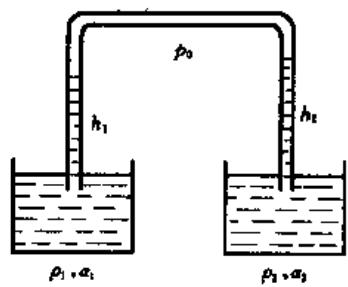
\includegraphics[width=0.2\textwidth]{figures/热图4-6-1.jpg}
\end{center}
\vfill

\newpage
\textbf{4-7} 已知水在1 atm和4 ℃时的表面张力系数 $\alpha = 7.24 \times 10^{-2} \, \mathrm{N/m}$ ，等温压缩系数 $\beta = -\frac{1}{V} \left( \frac{\partial V}{\partial p} \right)_T = 4.75 \times 10^{-5} \, \mathrm{atm}^{-1}$ 。若在1 atm和4 ℃时，水平液面下附近水的密度为 $\rho_0$ 。试问在1 atm和4 ℃时，半径 $r = 1.0 \times 10^{-6} \, \mathrm{cm}$ 的小水滴密度为多大？
\vfill

\textbf{4-8} 在连通管的两端吹出两个相同的球形肥皂泡A和B后，如热图4-8-1，关闭活栓K，活栓 $\mathbf{K}_{\mathrm{A}}$ 和 $\mathbf{K}_{\mathrm{B}}$ 则依旧打开，两泡内的空气经管相通，两泡相对平衡。

1.如热图 4-8-2，若 A 泡和 B 泡的形状小于半球，试证明 A 泡和 B 泡之间的平衡是稳定的。如热图4-8-3，若A泡和B泡的形状大于半球，试证明A泡和B泡之间的平衡是不稳定的。

2.若 A 泡和 B 泡的形状大于半球，设两管口的半径均为 $r_{1}=2.00\ \mathrm{cm}$ ，A 泡和 B 泡的半径均为 $r_{2}=2.50\ \mathrm{cm}$ 。试问当 A 泡和 B 泡分别变化成何种形状时，两泡能再次达到平衡。设空气因压缩或膨胀所引起的密度变化可以忽略。

\begin{center}
    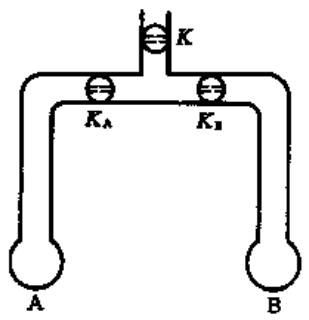
\includegraphics[width=0.1\textwidth]{figures/热图4-8-1.jpg}
    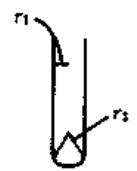
\includegraphics[width=0.1\textwidth]{figures/热图4-8-2.jpg}
    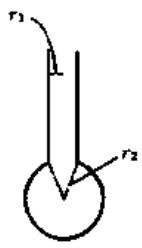
\includegraphics[width=0.1\textwidth]{figures/热图4-8-3.jpg}
\end{center}

\vfill

\newpage
\textbf{4-9} 如热图4-9-1，半径为 $R$ ，密度为 $\rho$ 的匀质球浮在 $0^{\circ}\mathrm{C}$ 的某液体表面上，球心高出液面 $h$。设球的热膨胀可以忽略。已知液体的热膨胀系数为 $\alpha$ ，表面张力系数 $\sigma$ 随摄氏温度 $t$ 的变化关系为 $\sigma(t) = \sigma_0(1 - \beta t)$ ，其中 $\beta$ 为常量。设液体对球为完全润湿。试证明，当系统温度小幅度变化时，球浸入液体部分体积不变的条件为
$$
\frac {\beta - \alpha}{\alpha} = \frac {2 R ^ {4} \rho g}{3 \sigma_ {0} (R ^ {2} - h ^ {2})}
$$
\begin{center}
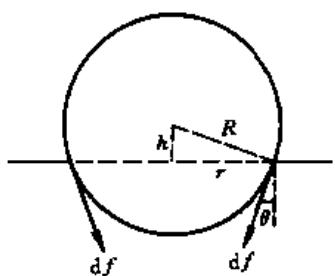
\includegraphics[width=0.2\textwidth]{figures/热图4-9-1.jpg}
\end{center}
\vfill

\textbf{4-10} 同一液体的两个球形膜碰在一起后，形成如热图4-10-1所示的对称连体膜。连体膜的两个球面（实际上是两个超过半球面的部分球面）的半径均为 $R$ ，中间相连的圆膜的半径为 $r$ ，圆膜边缘用一匀质细线围住。已知液体的表面张力系数为 $\sigma$ ，不计重力。试求细线内的张力 $T$ 。
\begin{center}
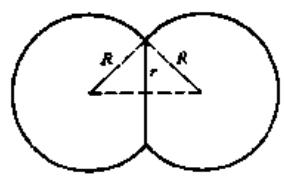
\includegraphics[width=0.2\textwidth]{figures/热图4-10-1.jpg}
\end{center}
\vfill

\newpage
\textbf{4-11} 将一竖直无限大平板部分地浸入与其有润湿作用的液体之中，两者之间的接触角为 $\theta$，液体密度为 $\rho$ ，表面张力系数为 $\alpha$ 。试求液体沿此板上升的高度。
\vfill

\textbf{4-12} 由同种原子组成的均匀一维晶体中，只有最相邻的原子之间有相互作用（余皆可略），作用势为 $V(x) = -\frac{A}{x^6} + \frac{B}{x^{12}}$ ，其中 $x$ 是相邻原子的间距， $A$ 和 $B$ 是两个常量。

1.试求平衡时原子间的平均距离。

2.当此晶体在平衡位置附近的相对形变为单位值时，试求其弹性倔强系数（用 A 和 B 表示）。

3.将晶体慢慢拉伸，试问当形变为多大时，晶体会被拉断。

\vfill

\newpage
\textbf{4-13} NaCl晶体在平衡态时 $\mathrm{Na}^{+}$ 和最邻近的 $\mathrm{Cl}^{-}$ 之间的距离为 $r_0 = 2.81\times 10^{-10}\mathrm{m}$ ，绝热压缩系数为 $k_{s} = -\frac{1}{V}\left(\frac{\mathrm{d}V}{\mathrm{d}p}\right)_{s} = 3.3\times 10^{-11}\mathrm{m}^{2} / \mathrm{N}$ ，马德隆常量为 $\alpha = 1.75$ 。试求平衡态时 $1\mathrm{mol}$ NaCl晶体的结合能 $E_{\mathrm{P0}}$ 。
\vfill

\textbf{4-14} 质量为 $2.0\mathrm{kg}$ ，温度为 $-13^{\circ}\mathrm{C}$ ，体积为 $0.19\mathrm{m}^{3}$ 的氟利昂（其分子量为121），在保持温度不变的条件下被压缩，体积减小为 $0.10\mathrm{m}^{3}$ 。试问在此过程中有多少千克的氟利昂被液化。已知在 $-13^{\circ}\mathrm{C}$ 时，液态氟利昂的密度为 $\rho = 1.44\times 10^{3}\mathrm{kg / m}^{3}$ ，饱和蒸汽压为 $p_{\text{饱}} = 2.08\times 10^{5}\mathrm{Pa}$ ，又氟利昂的饱和蒸汽可近似看作理想气体。
\vfill

\newpage
\textbf{4-15} 液体 $A, B$ 互不相溶，它们的饱和蒸汽压 $p$ 与温度 $T$ （绝对温标）的关系为
$$
\ln {\frac {p _ {i}}{p _ {0}}} = {\frac {a _ {i}}{T}} + b _ {i}, \quad i = A \text{ 或 } B
$$
其中 $p_0$ 是标准大气压， $a, b$ 是由液体本身性质确定的常量。测出两个温度的 $\frac{p_i}{p_0}$ 值如下：
$$
4 0 ^{\circ} \mathrm{C}, \quad \frac {p _ {A}}{p _ {0}} = 0. 2 8 4, \quad \frac {p _ {B}}{p _ {0}} = 0. 0 7 2 7 8
$$
$$
9 0 ^{\circ} \mathrm{C}, \quad \frac {p _ {A}}{p _ {0}} = 1. 4 7 6, \quad \frac {p _ {B}}{p _ {0}} = 0. 6 9 1 8
$$

1.在外部压强为 $p_0$ 时，试分别确定 $A$ 和 $B$ 的沸点。

2.现将 $100\mathrm{g}$ 液体 $A$ 和 $100\mathrm{g}$ 液体 $B$ 先后注入容器内，并在 $B$ 的表面覆盖上一薄层非挥发性液体 $C$，$C$ 与 $A$ 和 $B$ 互不相溶，$C$ 的作用是防止 $B$ 的自由蒸发。如热图4-15-1，各液层都不厚，因此液体内因重力产生的附加压强均可忽略。已知液体 $A$ 和 $B$ 的分子质量之比为 $\gamma = \frac{\mu_A}{\mu_B} = 8$ 。

缓慢而持续地加热容器，液体的温度 $t$ （摄氏温标）随时间 $\tau$ 的变化关系如热图 4-15-2 所示。试求出热图 4-15-2 中的温度 $t_1$ 和 $t_2$ （精确到 1℃），以及在 $\tau_1$ 时刻液体 A 和液体 B 的质量（精确到 0.1 g）。

\begin{center}
    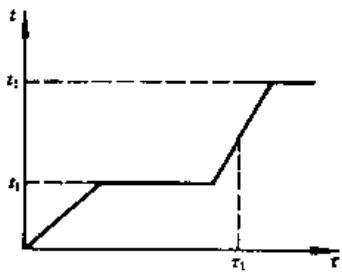
\includegraphics[width=0.3\textwidth]{figures/热图4-15-2.jpg}
    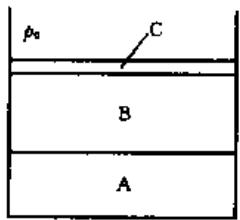
\includegraphics[width=0.3\textwidth]{figures/热图4-15-1.jpg}
\end{center}
设 A 和 B 的蒸汽均可看作理想气体，因而服从道尔顿分压定律。

\vfill
\newpage

\textbf{4-16} 在一密闭容器内有冰、水和水蒸汽各 $1\mathrm{g}$ ，三态共存达到平衡，系统的温度为 $t = 0.01$ ℃，压强为 $p = 4.58 \, \mathrm{mmHg}$ ，容器内别无其他物质。现在保持容器体积不变的条件下，对此系统缓慢加热，输入热量 $Q = 0.255 \, \mathrm{kJ}$ 。试估算此系统再次达到平衡后，冰、水和水蒸汽各自的质量。已知冰的升华热 $L_{\text{升}} = 2.83 \, \mathrm{kJ/g}$ ，水的汽化热 $L_{\text{汽}} = 2.49 \, \mathrm{kJ/g}$ 。
\vfill


\textbf{4-17} 地球深处 $35\mathrm{km}$ 到 $2900\mathrm{km}$ 之间的区域为固态地幔，地幔的主要成分是固态硅酸盐。设硅酸盐的熔解热为 $L_{m}$ ，其液态密度与固态密度之比为 $\alpha$ 。试求地幔中硅酸盐岩石的熔点 $T_{m}$ 随 $r$ 的变化率， $r$ 是岩石与地心的距离。

若已知地幔较上部位某处的 $T_{m}=1300\;^{\circ}\mathrm{C},\alpha=0.9,L_{m}=10^{5}\;\mathrm{cal/kg}$ 。试估算从该处往地心深入1000 m后， $T_{m}$ 变化了多少？
\vfill
